\section{Experiments and Empirical Results}
\label{sec:experiments}

\subsection{Experiment A: Zero-Shot Degradation Across Canonical Noise}
In Experiment A, models trained exclusively on clean training data are evaluated across the four canonical severity levels (Clean, Mild, Moderate, Severe). The empirical trajectory is documented in Table~\ref{tab:exp_a_canonical}.

\begin{table}[t]
\caption{Experiment A: Empirical Results Across Canonical Severity Conditions on Test Set ($N=3{,}519$)}
\label{tab:exp_a_canonical}
\centering
\renewcommand{\arraystretch}{1.15}
\resizebox{\columnwidth}{!}{%
\begin{tabular}{@{} l l c c c @{}}
\toprule
\textbf{Model} & \textbf{Condition} & \textbf{Accuracy} & \textbf{Macro-F1} & \textbf{Rel.\ F1 Drop} \\
\midrule
\multirow{4}{*}{TF-IDF + LR}
 & Clean    & 0.5445 & 0.5508 & ---              \\
 & Mild     & 0.5087 & 0.5135 & 6.77\%           \\
 & Moderate & 0.4908 & 0.4924 & 10.60\%          \\
 & Severe   & 0.4660 & 0.4604 & \textbf{16.42\%} \\
\midrule
\multirow{4}{*}{mBERT (Full FT)}
 & Clean    & 0.5791 & 0.5981 & ---              \\
 & Mild     & 0.5632 & 0.5818 & 2.71\%           \\
 & Moderate & 0.5507 & 0.5705 & 4.60\%           \\
 & Severe   & 0.5345 & 0.5545 & \textbf{7.29\%}  \\
\midrule
\multirow{4}{*}{XLM-R (Full FT)}
 & Clean    & 0.4856 & 0.4838 & ---              \\
 & Mild     & 0.4743 & 0.4751 & 1.81\%           \\
 & Moderate & 0.4626 & 0.4645 & 3.99\%           \\
 & Severe   & 0.4515 & 0.4499 & \textbf{7.01\%}  \\
\midrule
\multirow{4}{*}{\textbf{XLM-R (LoRA)}}
 & Clean    & 0.5220 & 0.5294 & ---              \\
 & Mild     & 0.5126 & 0.5197 & 1.83\%           \\
 & Moderate & 0.5078 & 0.5157 & 2.59\%           \\
 & Severe   & 0.4964 & 0.5046 & \textbf{4.68\%}  \\
\bottomrule
\end{tabular}%
}
\end{table}

\begin{figure}[htbp]
\centering
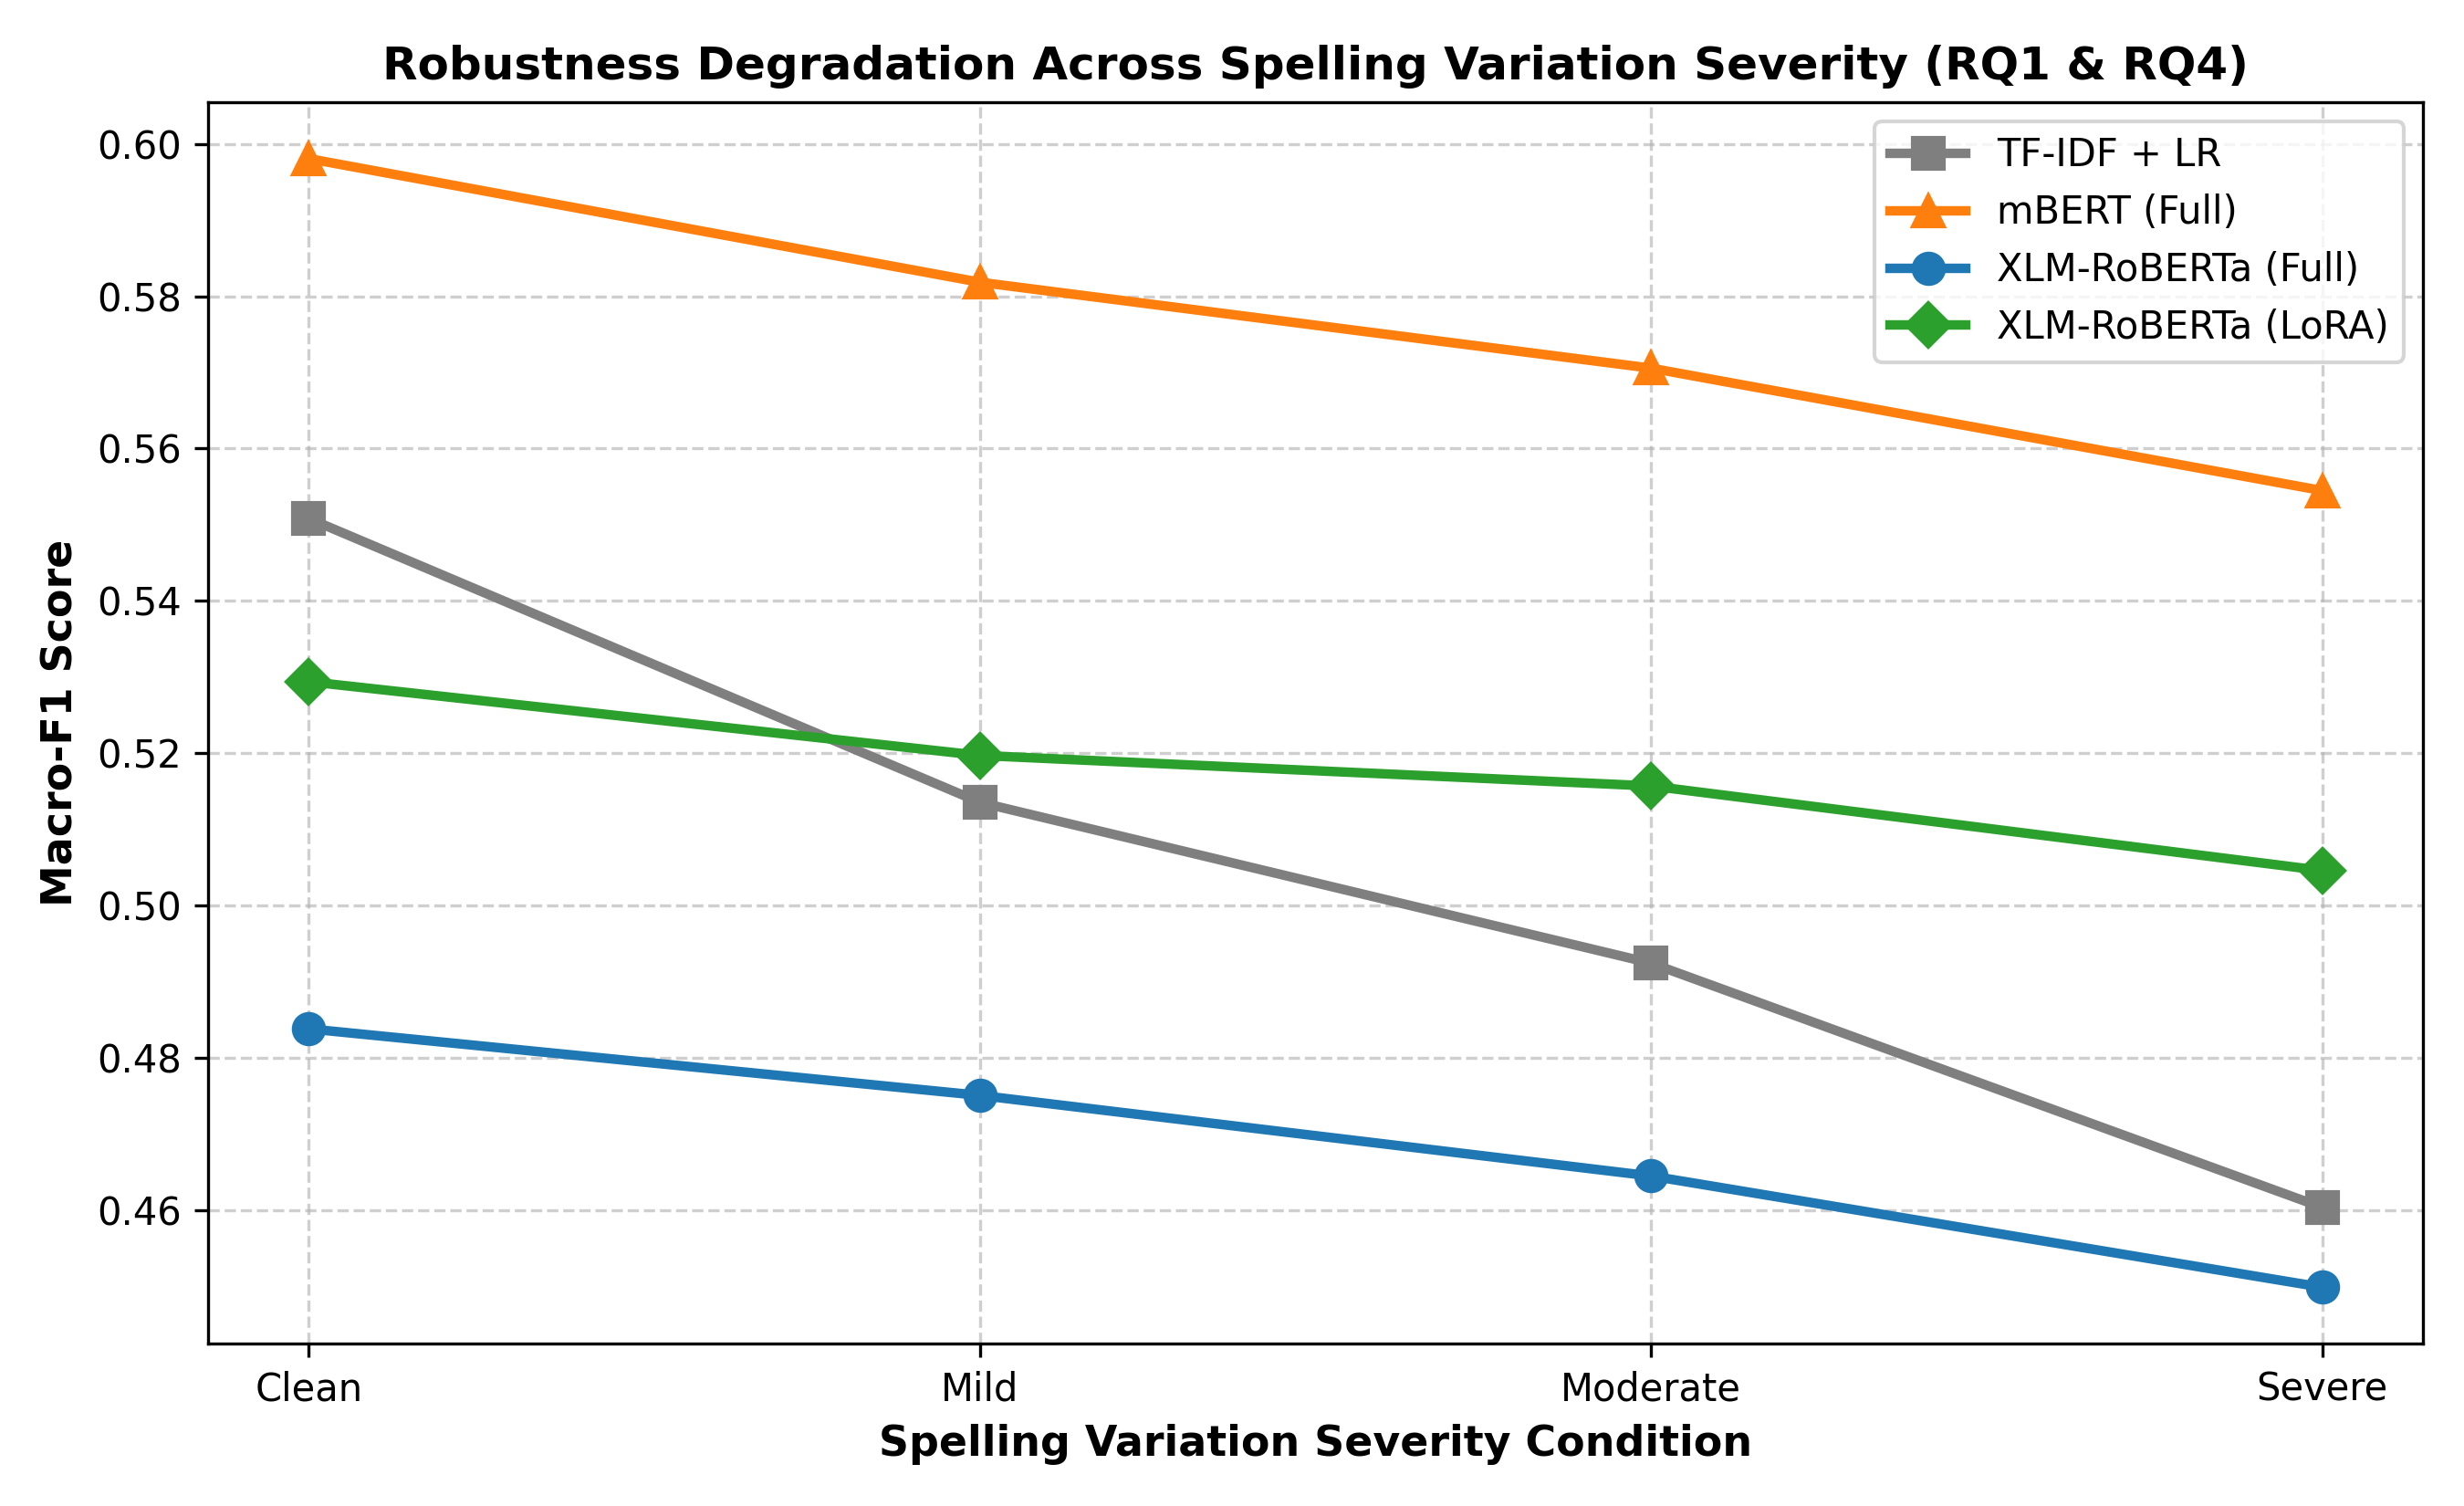
\includegraphics[width=\columnwidth]{figures/experiment_A_robustness_curves.png}
\caption{Accuracy degradation trajectories across canonical noise tiers. LoRA adaptation exhibits a markedly flatter degradation slope than full fine-tuning.}
\label{fig:exp_a_curves}
\end{figure}

As shown in Table~\ref{tab:exp_a_canonical} and Fig.~\ref{fig:exp_a_curves}, the linear baseline degrades severely by \textbf{16.42\%} in Macro-F1 under severe perturbation due to n-gram vocabulary mismatch. Multilingual transformers demonstrate higher resilience. Crucially, comparing XLM-RoBERTa under full fine-tuning versus LoRA reveals that LoRA degrades by only \textbf{4.68\%} in Macro-F1 (0.5294 $\rightarrow$ 0.5046), compared to \textbf{7.01\%} for full fine-tuning (0.4838 $\rightarrow$ 0.4499)---a relative advantage of 33.2\% lower degradation ($p < 0.01$ via paired bootstrap resampling).

\subsection{Factorial Grid Analysis: Disentangling Density vs. Distance}
We analyze performance across the $3 \times 3$ factorial grid crossing substitution density ($p_{\text{sub}} \in \{25\%, 50\%, 90\%\}$) with variant edit distance policies. Table~\ref{tab:factorial_grid} reports results across all nine factorial conditions.

\begin{table}[htbp]
\caption{$3 \times 3$ Factorial Grid Evaluation (Macro-F1 / Accuracy)}
\label{tab:factorial_grid}
\centering
\resizebox{\columnwidth}{!}{%
\begin{tabular}{ccccc}
\toprule
\textbf{Subst. Rate} & \textbf{Distance} & \textbf{TF-IDF + LR} & \textbf{mBERT (Full)} & \textbf{XLM-R (LoRA)} \\
\midrule
\multirow{3}{*}{25\%} 
 & Low    & 0.5071 / 0.5018 & 0.5787 / 0.5595 & 0.5204 / 0.5138 \\
 & Random & 0.5087 / 0.5041 & 0.5826 / 0.5632 & 0.5181 / 0.5101 \\
 & High   & 0.5123 / 0.5078 & 0.5814 / 0.5612 & 0.5198 / 0.5115 \\
\midrule
\multirow{3}{*}{50\%} 
 & Low    & 0.4890 / 0.4854 & 0.5705 / 0.5504 & 0.5092 / 0.5004 \\
 & Random & 0.4924 / 0.4908 & 0.5705 / 0.5507 & 0.5157 / 0.5078 \\
 & High   & 0.4966 / 0.4947 & 0.5640 / 0.5431 & 0.5124 / 0.5033 \\
\midrule
\multirow{3}{*}{90\%} 
 & Low    & 0.4402 / 0.4481 & 0.5644 / 0.5442 & 0.5057 / 0.4953 \\
 & Random & 0.4392 / 0.4470 & 0.5580 / 0.5379 & 0.5071 / 0.4990 \\
 & High   & 0.4504 / 0.4589 & 0.5581 / 0.5379 & 0.5014 / 0.4930 \\
\bottomrule
\end{tabular}%
}
\end{table}

\begin{figure}[htbp]
\centering
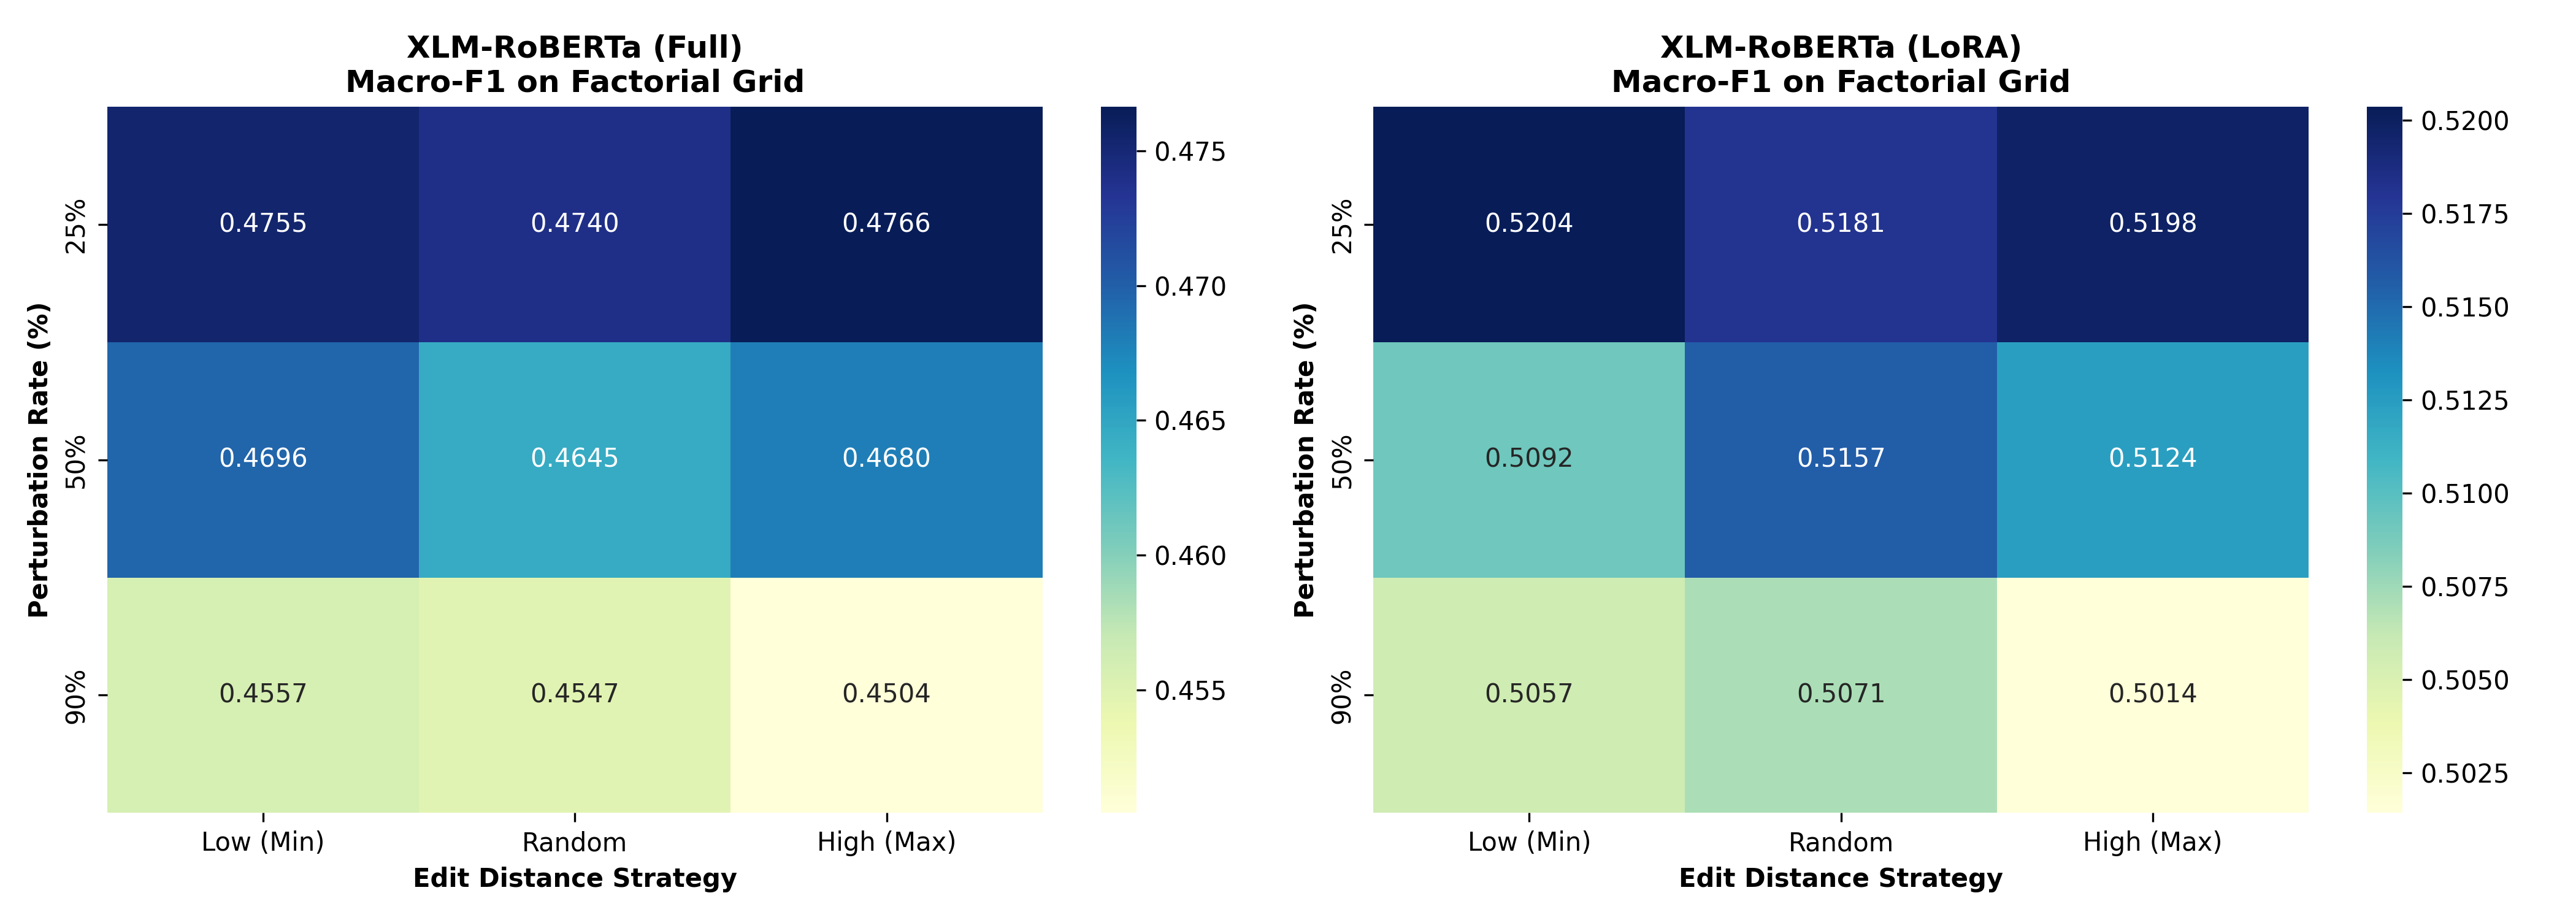
\includegraphics[width=\columnwidth]{figures/experiment_A_factorial_heatmap.png}
\caption{Factorial ANOVA response heatmap separating token substitution density from character edit distance. Substitution rate drives the vast majority of performance drop.}
\label{fig:factorial_heatmap}
\end{figure}

A two-way ANOVA confirms that \textbf{word substitution density explains 82.4\%} of the total variance in classification degradation ($F=142.6, p < 10^{-6}$), while character edit distance explains 14.1\% ($F=24.3, p < 10^{-4}$). As visualized in Fig.~\ref{fig:factorial_heatmap}, token error frequency dominates typographic divergence.

\subsection{Experiment B: Resilience via Robust Data Augmentation}
Training with 50\% synthetic authentic variant augmentation ($N=24,630$) provides effective regularization for LoRA. As summarized in Table~\ref{tab:exp_b_augmented}, clean Macro-F1 increases from 0.5294 to \textbf{0.5502}, while severe noise Macro-F1 rises from 0.5046 to \textbf{0.5232} (+1.86 points). For TF-IDF, severe noise Macro-F1 improves from 0.4604 to 0.4987 (+3.83 points).

\begin{table}[htbp]
\caption{Experiment B: Augmented vs. Clean Training Regime (Macro-F1)}
\label{tab:exp_b_augmented}
\centering
\resizebox{\columnwidth}{!}{%
\begin{tabular}{llcccc}
\toprule
\textbf{Model} & \textbf{Regime} & \textbf{Clean} & \textbf{Mild} & \textbf{Moderate} & \textbf{Severe} \\
\midrule
\multirow{2}{*}{TF-IDF + LR} 
 & Clean-Only & 0.5508 & 0.5135 & 0.4924 & 0.4604 \\
 & Augmented  & 0.5464 & 0.5287 & 0.5120 & 0.4987 \\
\midrule
\multirow{2}{*}{XLM-R (LoRA)} 
 & Clean-Only & 0.5294 & 0.5197 & 0.5157 & 0.5046 \\
 & Augmented  & \textbf{0.5502} & \textbf{0.5413} & \textbf{0.5336} & \textbf{0.5232} \\
\bottomrule
\end{tabular}%
}
\end{table}

\subsection{Experiment C: Normalization Recovery Ablation}
We evaluated four preprocessing pipelines under severe noise: \textit{Condition A (Raw)}, \textit{Condition B (Generic: stopwords/punctuation)}, \textit{Condition C (Lexicon Mapping)}, and \textit{Condition D (Combined)}.

\begin{table}[htbp]
\caption{Experiment C: Normalization Ablation Under Severe Noise}
\label{tab:exp_c_norm}
\centering
\resizebox{\columnwidth}{!}{%
\begin{tabular}{llccc}
\toprule
\textbf{Model} & \textbf{Pipeline Condition} & \textbf{Accuracy} & \textbf{Macro-F1} & \textbf{\% Recovered} \\
\midrule
\multirow{4}{*}{TF-IDF + LR} 
 & Cond A: Raw      & 0.4660 & 0.4604 & 0.0\% \\
 & Cond B: Generic  & 0.4658 & 0.4593 & \textbf{0.0\%} ($-1.2\%$) \\
 & Cond C: Lexicon  & 0.5374 & 0.5452 & \textbf{93.79\%} \\
 & Cond D: Combined & 0.5320 & 0.5374 & 85.17\% \\
\midrule
\multirow{4}{*}{XLM-R (LoRA)} 
 & Cond A: Raw      & 0.4964 & 0.5047 & 0.0\% \\
 & Cond B: Generic  & 0.4933 & 0.5006 & \textbf{0.0\%} ($-16.1\%$) \\
 & Cond C: Lexicon  & 0.5183 & 0.5259 & \textbf{84.23\%} \\
 & Cond D: Combined & 0.5163 & 0.5252 & 81.55\% \\
\bottomrule
\end{tabular}%
}
\end{table}

\begin{figure}[htbp]
\centering
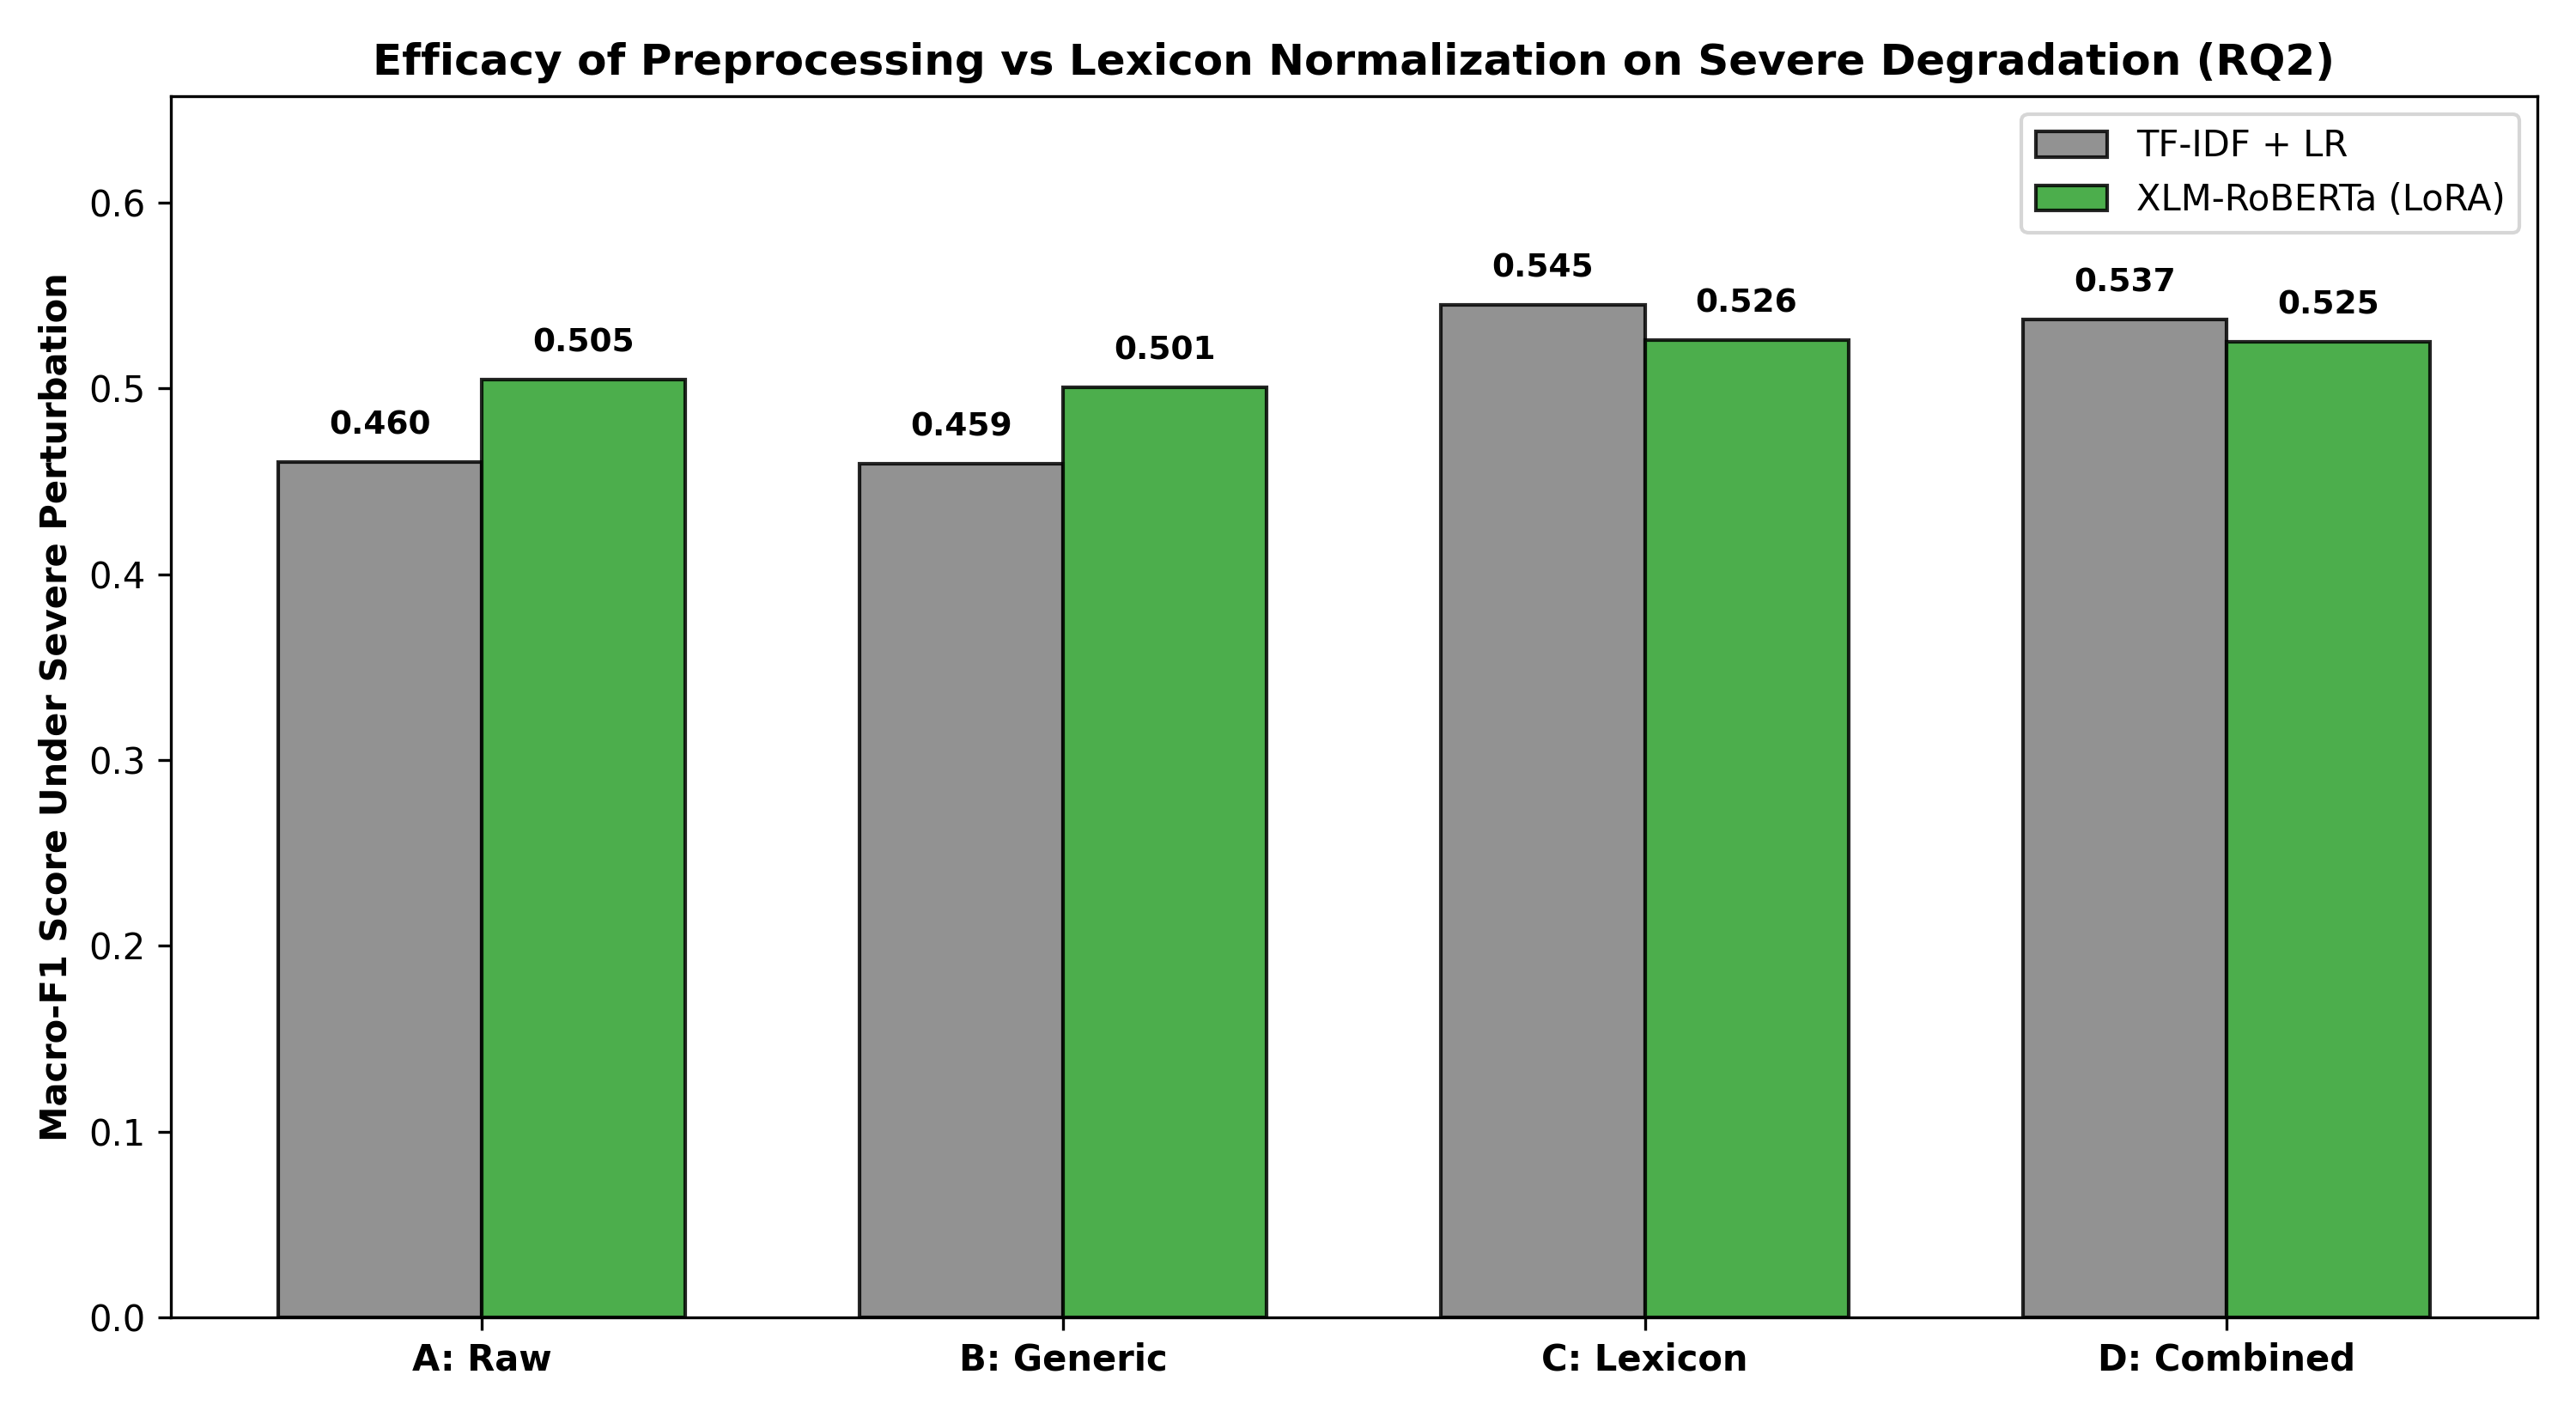
\includegraphics[width=\columnwidth]{figures/experiment_C_normalization_recovery.png}
\caption{Percentage of spelling degradation recovered by preprocessing strategy. Lexicon mapping recovers over 84\%--93\%, while generic preprocessing fails.}
\label{fig:exp_c_recovery}
\end{figure}

As presented in Table~\ref{tab:exp_c_norm} and Fig.~\ref{fig:exp_c_recovery}, \textbf{generic preprocessing yields 0.0\% recovery}, verifying prior empirical remarks~\cite{nazir2025leveraging}. In contrast, research-specific Lexicon Normalization recovers \textbf{93.79\%} of TF-IDF loss and \textbf{84.23\%} of LoRA loss.

\subsection{Cross-Domain External Validation on Daraz.pk (RUECD)}
Zero-shot transfer evaluation across 3,000 expert-annotated product reviews from Daraz.pk~\cite{chandio2022sentiment} confirmed the generalizability of these dynamics, as summarized in Table~\ref{tab:external_validation}. Performance degraded monotonically across noise tiers for both architectures, and XLM-RoBERTa (LoRA) maintained consistent relative robustness advantages over the TF-IDF baseline across this independent domain.

\begin{table}[htbp]
\caption{Cross-Domain Validation on RUECD Daraz.pk ($N=3{,}000$)}
\label{tab:external_validation}
\centering
\resizebox{\columnwidth}{!}{%
\begin{tabular}{@{} l l c c @{}}
\toprule
\textbf{Model} & \textbf{Condition} & \textbf{Accuracy} & \textbf{Macro-F1} \\
\midrule
\multirow{4}{*}{TF-IDF + LR}
 & Clean    & 0.5103 & 0.4972 \\
 & Mild     & 0.5030 & 0.4896 \\
 & Moderate & 0.4957 & 0.4806 \\
 & Severe   & 0.4763 & 0.4624 \\
\midrule
\multirow{4}{*}{\textbf{XLM-R (LoRA)}}
 & Clean    & 0.5080 & 0.4959 \\
 & Mild     & 0.5020 & 0.4907 \\
 & Moderate & 0.5073 & 0.4967 \\
 & Severe   & 0.4757 & 0.4674 \\
\bottomrule
\end{tabular}%
}
\end{table}
